\begin{figure*}[htbp]
\begin{subfigure}[b]{0.32\textwidth}
    \centering
    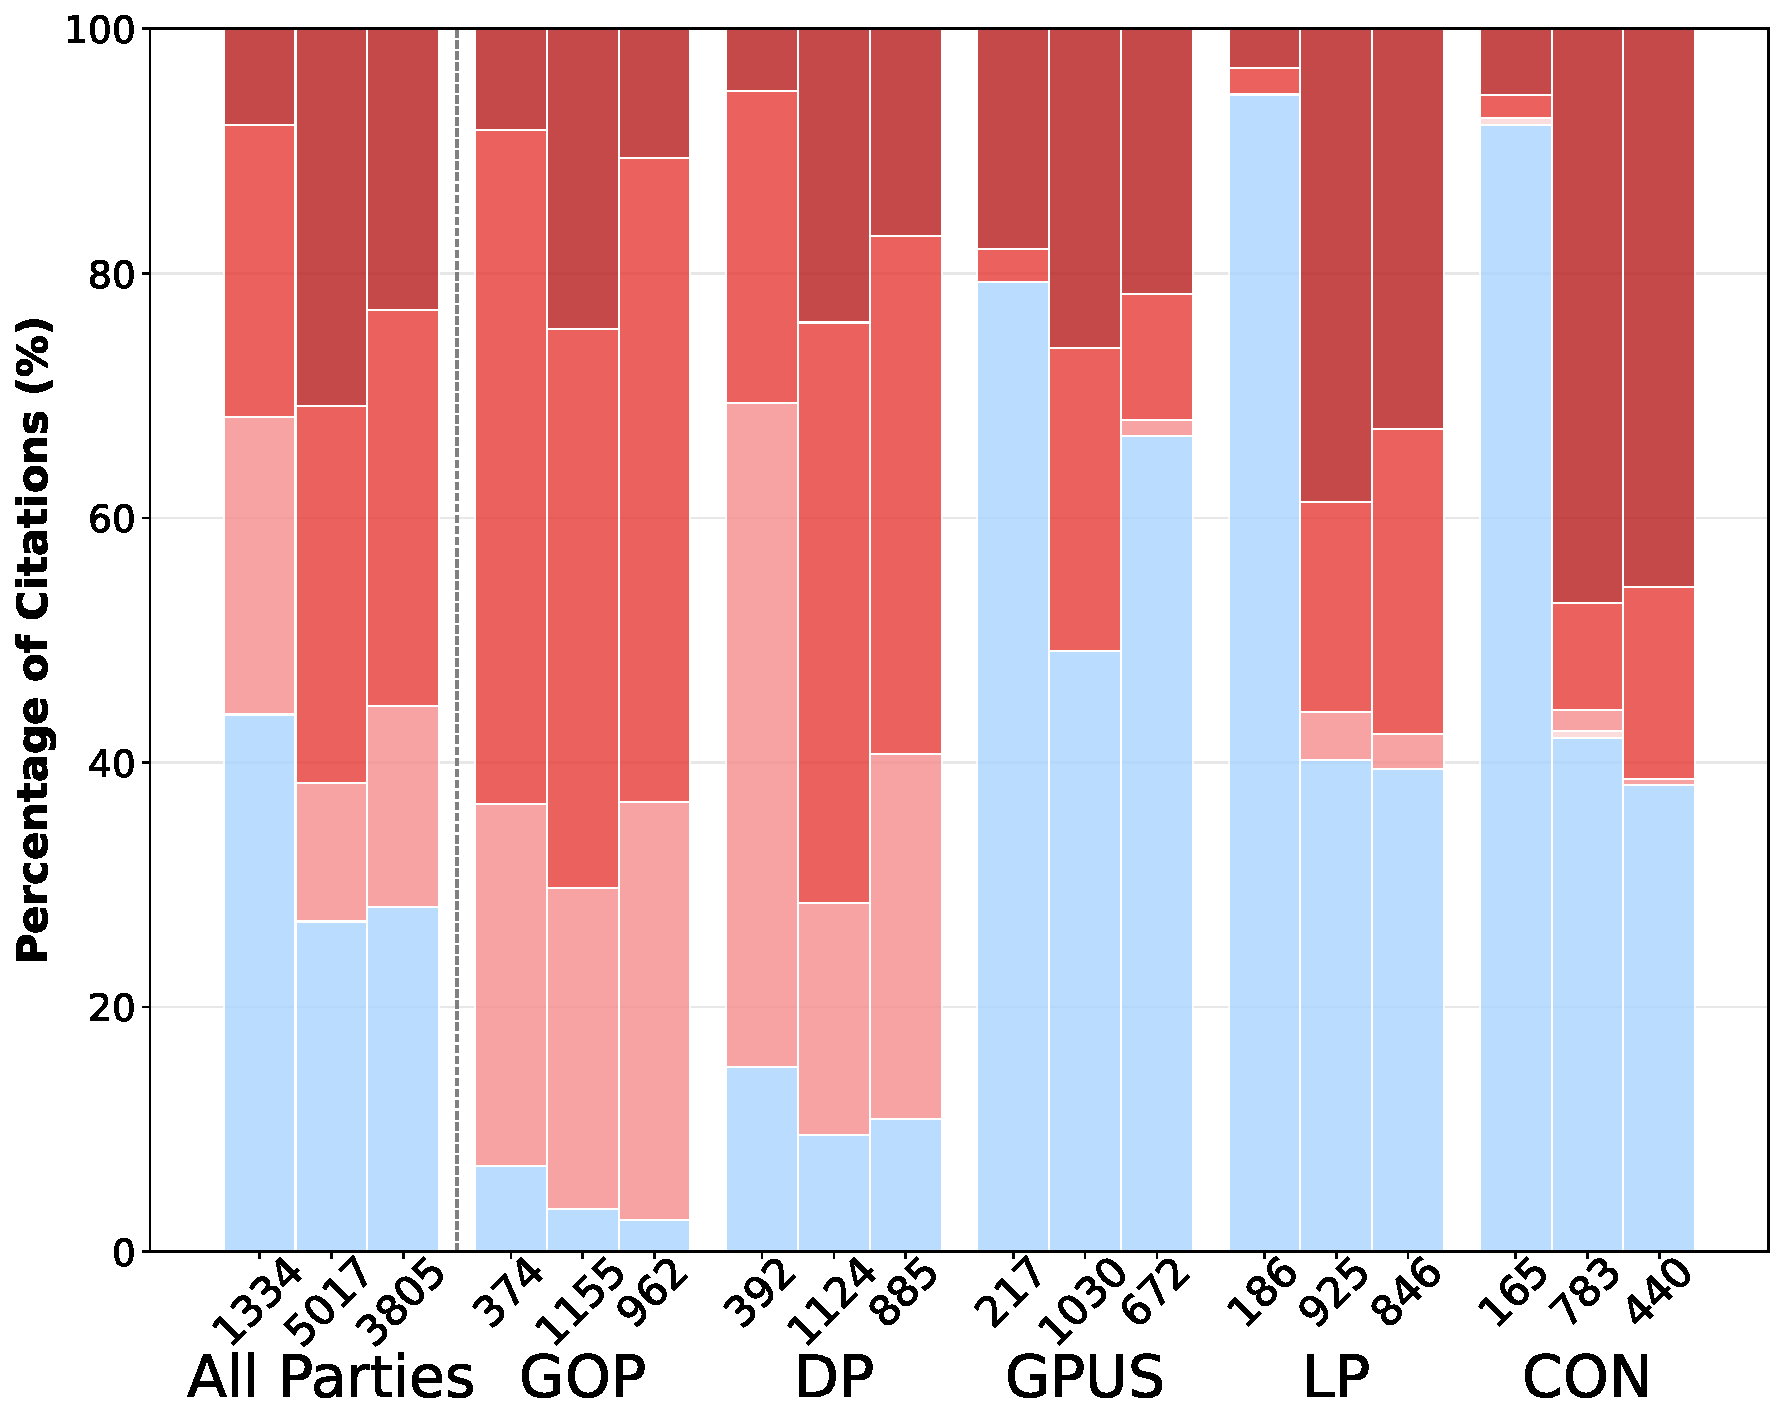
\includegraphics[width=\textwidth]{figs/US/all_parties_models_integrated_en_politics_prompts_red-blue.pdf}
    \caption{Citation Distributions (U.S.)}
    \label{fig:all_en}  
\end{subfigure}
\begin{subfigure}[b]{0.64\textwidth}
    \centering
    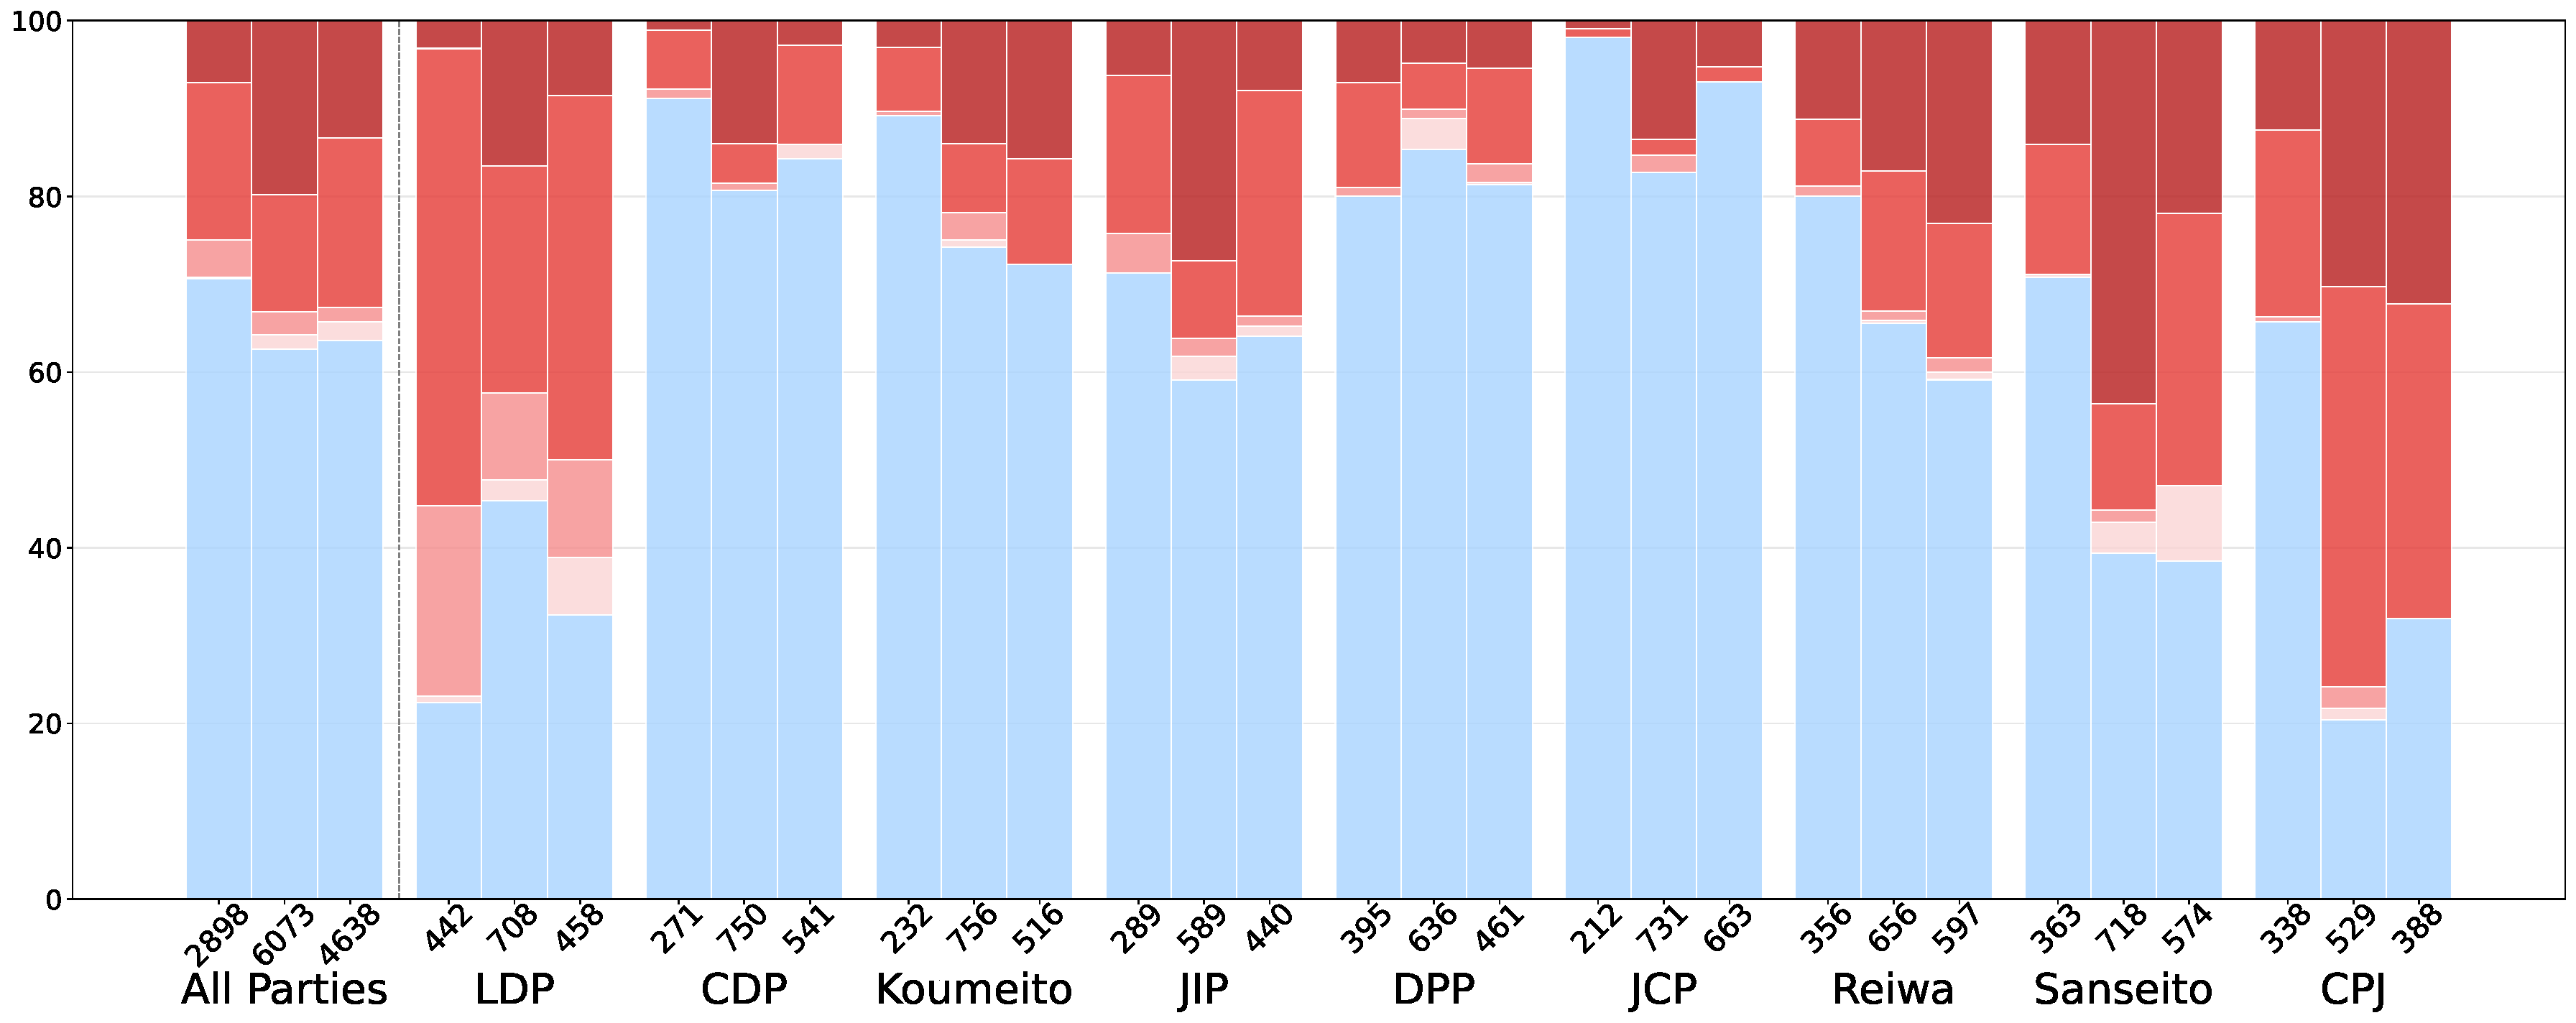
\includegraphics[width=\textwidth]{figs/JA/all_parties_models_integrated_ja_politics_prompts_red-blue.pdf}
    \caption{Citation Distributions (Japan)}
    \label{fig:all_ja}
\end{subfigure}
\begin{subfigure}[b]{0.99\textwidth}
    \centering
    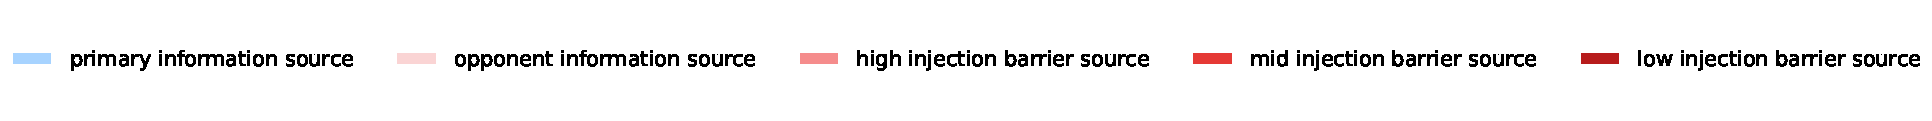
\includegraphics[width=\textwidth]{figs/full_legend.pdf}
\end{subfigure}
\caption{Distribution of citation sources by party in the US (a) and Japan (b): Each stacked bar shows the proportion of cited sources (primary, opponent, and secondary information sources categorized by attack cost) for responses generated by different APIs.
For each party, the three adjacent bars correspond to results from OpenAI (left), Gemini (middle), and Claude (right).
The three bars on the far right of each panel show aggregated results across all parties. The ``opponent source'' in All Parties chart reffers to the citation sources from parties that are not the target party for each question. The numbers under each chart shows the amout of total citation constructing it.}
\label{fig:party_wise}
\end{figure*}